%% "When you hear the name the Standard Model it sounds tedious and mundane, it should really be replaced by the Greatest Theory in the History of Human Civilization" - David Tong

\chapter{The Standard Model}
\label{chap:theory}

The Standard Model (SM) of particle physics is a rather simplistic name for such a powerful theory. It is the closest theory that exists to a complete description of the universe at the most fundamental level, and is arguably the pinnacle of science. In this chapter, the aim is to provide a a brief overview of the SM, relying on the derivations of Reference~\cite{Griffiths:2008zz}. For a more comprehensive description, one may refer to the above reference.

\section{Particle content}
\label{sec:particlecontent}

The Standard Model is often depicted in compact diagrams similar to that of Mendeleev's Periodic Table of Elements. One such diagram is shown in Figure \ref{fig:SM}. In a nutshell, the particles put forward by the SM are truly elementary particles. Unlike the elements in the Periodic Table which can be further broken down, these elementary particles are (to our knowledge) point-like and contain no internal structure. Each particle has a unique set of properties - quantum numbers - that define it, and split into one of two categories: fermions and bosons. 

Fermions are half-integer spin particles, and are usually thought of as matter particles. Each fermion has an anti-particle, with an identical mass but opposite electric charge. They are further classified as either leptons or quarks. Leptons are either negatively charged (-1), or neutral. The latter are referred to as neutrinos, which the SM predicts to be massless. Quarks have an electric charge of either $\frac{2}{3}$ or $\frac{-1}{3}$, and carry an additional colour charge of either red, blue, or green. The arrangement of fermions in the SM is generational. The first generation is found in everyday matter; for example the proton and neutron are made up of up and down quarks, and the electron which orbit nuclei. The second and third generation leptons have higher masses, but they otherwise behave identically. 

Bosons are integer spin particles that mediate the interactions within the SM. Electromagnetism is arguably the most well-known forces, and is carried by the massless and chargeless photon $\gamma$. Electric charge is conserved during photon-mediated particle interactions, and the photon has infinite range. that Eight gluons mediate the strong force of quantum chromodynamics. They are also massless and electromagnetically neutral, but carry a colour charge. Only quarks are able to interact with gluons, and they can self-interact. Unlike the photon, however, gluons have finite range; as interaction distance increase, the interaction strength decreases. The weak force arises from the exchange of three massive force carriers: two charged $W^{\pm}$ bosons and a neutral $Z$ boson. As its name suggests, the force is relatively weak compared to the EM and strong forces, and is only carried over short ranges. The photon, $W^{\pm}$, and $Z$ bosons are gauge bosons of spin 1. Completing the SM is the spin 0 scalar Higgs boson. The Higgs is electrically neutral, colourless, and massive. It plays a key role in the SM by providing mass to gauge bosons and fermions through electroweak symmetry breaking.

\input{Content/SM_tikz}%\subsubsection{Fermions}
%
%Fermions are half-interger spin particles that are further divided into two groups due to their radically different properties. 

\section{Gauge fields}

The Standard Model is constructed upon the language of quantum field theory, where every elementary particle is described as quantizations \todo{(pertubations?)} of a quantum field. It describes the strong and electroweak interaction from the $\SUgroup3_C\otimes\SUgroup2_L\otimes\Ugroup1_Y$ symmetry group, each with a conserved quantity (following Noether's theorem) as indicated by the indices. All the interactions of the SM can be derived on the basis that the system is invariant under local gauge transformations. Imposing local gauge invariance under \SUgroup{3} and colour charge conservation returns Quantum Chromodynamics (QCD). 

\subsection{Quantum electrodynamics}
\label{ssec:QED}

The Dirac Lagrangian, written as
\begin{equation} \label{eq:diracfreelagr}
    \Lagrangian=i\hbar c\bar{\psi}\gamma^{\mu}\partial_{\mu}\psi-mc^2\bar{\psi}\psi
\end{equation}
is invariant under a global gauge transformation $\psi\rightarrow e^{i\theta}\psi$, but not under a local gauge transformation where $\theta$ is a function of $x^{\mu}$. In order for the Lagrangian to be complete an additional term must be added to equation \ref{eq:diracfreelagr}. 
\begin{equation} \label{eq:diraclagr}
    \Lagrangian=i\hbar c\bar{\psi}\gamma^{\mu}\partial_{\mu}\psi-mc^2\bar{\psi}\psi-q\bar{\psi}\gamma^{\mu}\psi A_{\mu}
\end{equation}
This term introduces a new gauge field $A_{\mu}$, which transforms under local gauge transformations in a way that renders equation \ref{eq:diraclagr} invariant. This is not yet complete, since the new vector field must include it's own "free" term - the Proca Lagrangian
\begin{equation} \label{eq:proclagr}
    \Lagrangian=\dfrac{-1}{16\pi}F^{\mu\nu}F_{\mu\nu}+\dfrac{1}{8\pi}\Big(\dfrac{m_Ac}{\hbar}\Big)^2 A^{\nu}A_{\nu}
\end{equation}
where it can be seen that the gauge field must be massless, because $A^{\nu}A_{\nu}$ is not invariant under local gauge transformation $A_{\mu}\rightarrow A_{\mu}+\partial \lambda$. Also introduced in equation \ref{eq:proclagr} is the shorthand 
\begin{equation}
    F^{\mu\nu}\equiv\partial^{\mu}A^{\nu}-\partial^{\nu}A^{\mu}.
\end{equation}
To summarise, in requiring local gauge invariance from the Dirac Lagrangian, a vector field with no mass is introduced. Indeed, this vector field is the field of the massless photon.
\begin{equation}\label{eq:QEDlagr}
    \Lagrangian=i\hbar c\bar{\psi}\gamma^{\mu}\partial_{\mu}\psi-mc^2\bar{\psi}\psi+\dfrac{-1}{16\pi}F^{\mu\nu}F_{\mu\nu}-q\bar{\psi}\gamma^{\mu}\psi A_{\mu}
\end{equation}

Going back to the free Dirac Lagrangian in equation \ref{eq:diracfreelagr}, what if an alternate definition of the derivative, namely 
\begin{equation}
    \mathcal{D}_{\mu}\equiv \partial_{\mu}+i\dfrac{q}{\hbar c}A_{\mu}
\end{equation}
were to replace $\partial_{\mu}$? Suppose as well that $\mathcal{D}_{\mu}$, hereforth referred to as the covariant derivative, transforms like the field $\psi$ itself:
\begin{equation}
    \mathcal{D}_{\mu}\psi\rightarrow e^{i\theta(x_{\mu})}\mathcal{D}_{\mu}\psi .
\end{equation}
\todo[inline]{Read more into this, and derive it on paper? A bit confused as to how it works out.}
It turns out that in doing so, the transformation of of $A_{\mu}$, 
\begin{equation}
    A_{\mu}\rightarrow A_{\mu}-\dfrac{\hbar c}{q}\partial_{\mu}\theta
\end{equation}
renders the Lagrangian locally invariant. $A_{\mu}$ brings along its own free Lagrangian, however, and the field must be massless to preserve local gauge invariance. All together this give the final Lagragian stated in equation \ref{eq:QEDlagr}, describing the interactions of fermions with charge $q$ (Dirac fields) with photons (Maxwell fields), more commonly known as the Lagrangian for quantum electrodynamics. 

\subsection{Quantum chromodynamics}

The coloured quark model dictates that each flavour (six in total) comes in three identical variations. Arbitrarily, colour is used to differentiate between these variations: for each quark flavour, there exists a red, blue, and green version. The quark field in its colour triplet is written in vector notation as
\begin{equation}
\psi_q\equiv
    \begin{pmatrix} 
        \psi_q^r\\ 
        \psi_q^b\\
        \psi_q^g
    \end{pmatrix}
,\quad
\bar{\psi}_q=(\bar{\psi}_q^r,\bar{\psi}_q^b,\bar{\psi}_q^g)
\end{equation}
such that the Lagrangian resembles the free Dirac Lagragian,
\begin{equation} \label{eq:QCDfreelagr}
    \Lagrangian=i\bar{\psi}_q\gamma^{\mu}\partial_{\mu}\psi_q-m^2\bar{\psi}_q \psi_q.
\end{equation}
\todo[inline]{Some stuff to fill in... see page 355-356 of Griffiths}

The Lagrangian must be modified to maintain local gauge invariance under \SUgroup{3} gauge transformations of the form
\begin{equation}
    \psi_q\rightarrow S\psi_q=e^{i\lambda_a\theta^a}\psi_q.
\end{equation}
As with the case in QED, a covariant derivative is introduced to replace the ordinary derivative:
\begin{equation}
    \mathcal{D}_{\mu}\equiv \partial_{\mu}+ig_s\lambda_a{G^a_{\mu}}\\
\end{equation}
where $\lambda_a$ with $a=1,2,...,8$ are the Gell-Mann $3\times3$ matrices, whose role for \SUgroup{3} is the role Pauli spin matrices play for \SUgroup{2}. For the new gauge fields $G^a$, the transformation rule considering the infinitesimal case is 
\begin{equation}
    G^a_{\mu}\rightarrow G^a_{\mu}-\dfrac{1}{g_s}\partial_{\mu}\theta_a-f_{ijk}\theta^jG_{\mu}^k
\end{equation}
where $f_{ijk}$ are the structure constants of \SUgroup{3}. 

The modified Lagrangian (with the covariant derivative replacing the derivative) ins locally invariant under \SUgroup{3} transformations, and consequently eight new gauge fields are introduced. Unsurprisingly, these correspond precisely to the eight gluons. Lastly, the Proca-Lagrangian for the gluon fields must be added in. Here it is useful to define
\begin{equation}
    G^{\mu\nu}_a \equiv \partial^{\mu}G_a^{\nu}-\partial^{\nu}G_a^{\mu}-g_sf_{ijk}G^{\mu}_jG^{\nu}_k
\end{equation}
so that the final Lagrangian describing quantum chromodynamics is
\begin{equation}
    \Lagrangian=[i\bar{\psi}\gamma^{\mu}\partial_{\mu}\psi-m\bar{\psi}\psi] - \dfrac{1}{4}G^{\mu\nu}_aG^a_{\mu\nu}-g_s\bar{\psi}\gamma^{\mu}\lambda_a \psi G_{\mu}^a
\end{equation}

\subsection{Weak interactions and electroweak unification}

%\todo[inline]{In addition to the linked thread: A SU(2) doublet is a pair of states (particles) which can be rotated into each other by SU(2) (gauge) transformations. You have weak isospin (T3) up and down, but you are free to e.g. replace up <-> down everywhere without changing the physics. A singlet has no SU(2) "charge" and it not affected by the transformation. In the SM, left-handed leptons are SU(2) doublets  and right-handed ones SU(2) singlets . In the same way, you have color triplets (quarks), singlets (leptons), and octets (gluons) under SU(3).}

The global gauge transformation $\psi\rightarrow e^{i\theta}\psi$ where $\theta$ is any real number can be though of as a matrix multiplication of the form
\begin{equation}
    \psi\rightarrow U\psi
\end{equation}
where $U^{\dag}U=1$ and in this case $U=e^{i\theta}$. The group of all possible unitary $1\times1$ matrices is called $\Ugroup{1}$. The same logic was applied in 1954 by Yang and Mills to the \SUgroup{2} group.

% The weak interaction theory is described using the non-abelian\todo{Describe non-abelian} symmetry group SU(2). In analogy with the formalism of QCD the generators of the group give rise to the gauge fields. In QCD there are eight generators, the Gell-Mann matrices, that give rise to the introduction of eight gauge fields identified as gluons. Similarly, in the weak theory there are three generators, the Pauli-spin matrices, that give rise to three gauge fields identified as the Z 0 , W+ and W− vector bosons. According to Noether’s theorem4 , a quantity or current is conserved providing gauge invariance is shown. For example, in QED the electric charge is conserved and in QCD it is colour charge that is conserved. In the case of the weak interaction, the conserved quantity is called weak isopin, T1,2.3.

Experimental observations have shown that weak charged currents couple only to left-handed fermions and right-handed anti-fermions \cite{Pich:2007vu}. In order to extract the left- and right-handed components, it is useful to define the projection operators $P_L$ and $P_R$, which act on fermion fields (expressed by Dirac spinors) in the following manner:
\begin{equation}
    \psi_{L}=P_{L}\psi=\dfrac{1}{2}(1- \gamma_5)\psi,\quad 
    \psi_{R}=P_{R}\psi=\dfrac{1}{2}(1+ \gamma_5)\psi
\end{equation}

The left-handed and right-handed fermion fields follow different definitions under \SUgroup{2}. The former are arranged as doublets with isospin $I=\frac{1}{2}$, while the latter are singlets with isospin $I=0$. The singlets are consequently unaffected by \SUgroup{2} local gauge transformation.
\begin{align}\label{eq:SU2doublet}
    \ell_L & =
    \begin{pmatrix}
        \nu_e\\
        e
    \end{pmatrix}_L,
        \begin{pmatrix}
        \nu_{\mu}\\
        \mu
    \end{pmatrix}_L,
        \begin{pmatrix}
        \nu_{\tau}\\
        \tau
    \end{pmatrix}_L
    & q_L & =
    \begin{pmatrix}
        u\\
        d'
    \end{pmatrix}_L,
    \begin{pmatrix}
        c\\
        s'
    \end{pmatrix}_L,
    \begin{pmatrix}
        t\\
        b'
    \end{pmatrix}_L\\
    \ell_R & =e_R, \quad \mu_R, \quad \tau_R
    \qquad 
    & q_R & = u_R, \quad d_R, \quad c_R, \quad s_R, \quad t_R, \quad b_R
\end{align}
Notice that in equation \ref{eq:SU2doublet} the the down type quark doublet partners are weak eigenstates that can transform into one another through interactions with $W$ bosons \cite{Raby:1997bp}. The weak eigenstates $d'$, $s'$ and $b'$ are related to the mass eigenstates $d$, $s$ and $b$ through a unitary $3\times3$ matrix - the Cabbibo-Kobayashi-Maskawa (CKM) matrix. 
\begin{equation}
    \begin{pmatrix}
        d'\\
        s'\\
        b'
    \end{pmatrix}
    =
    \begin{pmatrix} 
        V_{ud} && V_{us} && V_{ub}\\ 
        V_{cd} && V_{cs} && V_{cb}\\
        V_{td} && V_{ts} && V_{tb}
    \end{pmatrix}
        \begin{pmatrix}
        d\\
        s\\
        b
    \end{pmatrix}
\end{equation}

Similar to the QED and QCD case, a covariant derivative $\mathcal{D}_{\mu}$ is defined for the theory to retain its invariance under local gauge transformations:
\begin{equation}
    \mathcal{D}_{\mu}\equiv \partial_{\mu}+ig_W\dfrac{\sigma^a}{2}W^a_{\mu}+ig'\dfrac{Y}{2}B_{\mu}
\end{equation}
where $g$ and $g'$ represent the weak coupling constants, $\sigma_a$ with $a=1,2,3$ are the pauli matrices (i.e. the generators of \SUgroup{2}), and $Y$ is the weak hypercharge (generator of \Ugroup{1}). $Y$ is the conserved quantity from the $\Ugroup{1}_Y$ symmetry and it is related to the electric charge $Q$ by
\begin{equation}
    Q=T_3+\dfrac{Y}{2}
\end{equation}
where $T_3$ is the third component of weak isospin.
The Pauli matrices satisfy the condition
\begin{equation}
    [\sigma_a,\sigma_b]=2i\epsilon_{abc}\sigma^c.
\end{equation}

In defining the covariant derivative, four new massless gauge fields $W^1_{\mu}, W^2_{\mu}, W^3_{\mu}$ and $B_{\mu}$ are introduced. The former corresponds to the three \SUgroup{2}$_L$ generators, while the latter is associated with \Ugroup{1}$_Y$. The mixing of these four fields gives the electroweak bosons $W^+,W^-,Z$ and $\gamma$. The charged bosons $W^+$ and $W^-$ are linear combinations of $W^1_{\mu}$ and $W^2_{\mu}$:
\begin{align}
    W^+_{\mu} & =\dfrac{1}{\sqrt{2}}(W_{\mu}^1-iW_{\mu}^2)\\
    W^-_{\mu} & =\dfrac{1}{\sqrt{2}}(W_{\mu}^1+iW_{\mu}^2).
\end{align}
The remaining fields $W_{\mu}^3$ and $B_{\mu}$ combine to form the Z boson and the photon as follows:
\begin{align}
    A_{\mu} & =B_{\mu}\cos\theta_{w}+W^3_{\mu}\sin\theta_w\\
    Z_{\mu} & =-B_{\mu}\sin\theta_{w}+W^3_{\mu}\cos\theta_w
\end{align}
where $\theta_w$ denotes the Weinberg angle.

The field strength tensors for \SUgroup{2}$_L$ and \Ugroup{1}$_Y$ are defined as: 
\begin{align} \label{eq:EWKtensors}
    W^a_{\mu\nu} & =\partial_{\mu}W^a_{\nu}-\partial_{\nu}W^a_{\mu}-g\epsilon^{abc}W^b_{\mu}W^a_{\nu}\\
    B_{\mu\nu} & =\partial_{\mu}B_{\nu}-\partial_{\nu}B_{\mu}
\end{align}.
The first line of equation \ref{eq:EWKtensors} is reminiscent of QCD, where last term gives rise to self-couplings of the electroweak gauge bosons. 

The electroweak interaction, invariant under \SUgroup{2}$_L\times$\Ugroup{1}$_Y$ gauge transformations, has the following Lagrangian:
\begin{equation}
    \Lagrangian=\sum_{j}i\bar{\psi}_j\gamma^{\mu}\mathcal{D}_{\mu}\psi_j-\dfrac{1}{4}B_{\mu\nu}B^{\mu\nu}-\dfrac{1}{4}W^a_{\mu\nu}W_a^{\mu\nu}
\end{equation}
where $j$ iterates over all the fermion fields. The requirement of local gauge invariant led to the construction of this Lagrangian that unifies the electromagnetic and weak interactions, from which the the physical interactions between fermions and the electroweak gauge bosons are correctly reproduced. The electroweak Lagrangian above, however, does not allow for gauge field mass terms. While the photon (and the gluon) is indeed massless, the fermions, $W$, and $Z$ bosons have been experimentally shown to be massive \cite{missing}. This is an inconsistency that urgently needs addressing - luckily, there is a way to reform gauge theory to accommodate massive gauge fields. 

\section{Spontaneous symmetry breaking and the Higgs mechanism} \label{sec:SSBHiggsMechanism}
\subsection{Spontaneous symmetry breaking}\label{ssec:SSB}
\subsubsection{Broken discrete symmetry}

The Lagrangian written in the classic form of a kinetic term minus a potential term, is:
\begin{align}
    \Lagrangian & = T-V\\
    \Lagrangian & = \dfrac{1}{2}(\partial_{\mu}\phi)(\partial^{\mu}\phi)-(\dfrac{1}{2}\mu^2\phi^2+\dfrac{1}{4}\lambda\phi^4).
    \label{eq:ssbLagrangian}
\end{align}
For the potential to have a finite minimum, $\lambda$ must be positive. The minimum of the potential $V(\phi)$ occurs at 
\begin{equation}
    \phi=\pm\sqrt{\dfrac{-\mu^2}{\lambda}}
\end{equation}
A new field can be written as perturbations from the ground states, defined by 
\begin{equation}
    \eta\equiv\phi\pm\sqrt{\dfrac{-\mu^2}{\lambda}}.
\end{equation}
If the Lagrangian of equation \ref{eq:ssbLagrangian} is rewritten in terms of $\eta$ as
\begin{equation} \label{eq:ssbReformedLagrangian}
    \Lagrangian=\dfrac{1}{2}(\partial_{\eta}\phi)(\partial^{\eta}\phi) - \mu^2\eta^2\pm\mu\lambda\eta^3-\dfrac{1}{4}\lambda\eta^4+\dfrac{1}{4}\dfrac{\mu^4}{\lambda}
\end{equation}
then the second term resembles a mass term, where the mass of the particle is 
\begin{equation}
    m=\sqrt{-2\mu^2}
\end{equation}
the third and fourth term of equation \ref{eq:ssbReformedLagrangian} represent triple and quartic couplings, and the last term is an insignificant constant. 
\begin{figure}[htp]
    \centering
    \resizebox{.5\textwidth}{!}{
    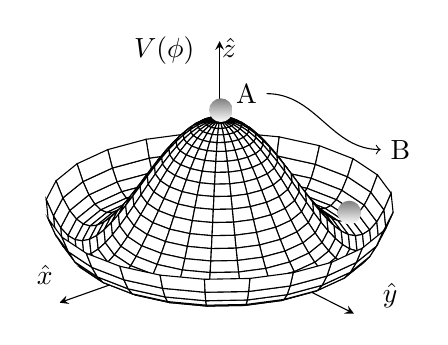
\begin{tikzpicture}
      \begin{axis}[
          axis lines=center,
          view={140}{25},
          axis equal,
          domain=0:360,
          y domain=0:1.25,
          xmax=1.5,ymax=1.5,zmin=0,zmax=1.5,
          x label style={at={(axis description cs:0.18,0.29)},anchor=north},
          y label style={at={(axis description cs:0.82,0.25)},anchor=north},
          z label style={at={(axis description cs:0.44,0.8)},anchor=north},
          xlabel = $\hat{x}$,
          ylabel=$\hat{y}$,
          zlabel=$V(\phi)\quad \hat{z}$,
          ticks=none,
          clip bounding box=upper bound
        ]
    
        \addplot3 [surf, shader=flat, draw=black, fill=white, z buffer=sort] ({sin(x)*y}, {cos(x)*y}, {(y^2-1)^2});
      \end{axis}
      \shade (3.47,3.5) circle [radius=0.15cm];
      \shade (5.1,2.2) circle [radius=0.15cm];
      \node[anchor=east] at (4.05,3.71) (text) {A};
      \node[anchor=west] at (5.5,3.0) (description) {B};
      \draw (description) edge[out=180,in=0,<-] (text);
    \end{tikzpicture}
    }
    \caption{Illustration of the Higgs potential. There is an infinite number of ground states. At point A, the global symmetry is unbroken. At point B, a local minimum is chosen and spontaneous symmetry breaking occurs. This figure is from Ref.~\cite{higgspotential}.}
    \label{fig:Higgspotential}
\end{figure}
\subsubsection{Broken continuous symmetry}

The previous section illustrates an example of spontaneous symmetry breaking. The original Lagrangian of equation \ref{eq:ssbLagrangian} is invariant if $phi\rightarrow-\phi$; it is even in $\phi$. In the reformed Lagrangian of equation \ref{eq:ssbReformedLagrangian}, however, this symmetry is broken because it is not even in $\eta$. The breaking is considered spontaneous because no external agent is required; the symmetry simply becomes hidden when selecting a particular ground state (the "vacuum"). In section \ref{sec:SSB} the broken symmetry was a discrete symmetry in context of a read scalar field. This section will apply spontaneous symmetry breaking to a complex scalar field.

Consider the following complex scalar field, written neatly as a combination of two real fields:
\begin{equation}
    \phi\equiv\dfrac{1}{\sqrt{2}}(\phi_1+i\phi_2)\\ \label{eq:complexfield}
    \phi^*\phi=\dfrac{1}{2}(\phi^2_1+\phi^2_2).
\end{equation}
The Lagrangian written with respect to the two fields $\phi_1$ and $\phi_2$ is
\begin{equation}\label{eq:SSBContLagrangian}
    \Lagrangian=\dfrac{1}{2}(\partial_{\mu}\phi_1)(\partial^{\mu}\phi_1) + \dfrac{1}{2}(\partial_{\mu}\phi_2)(\partial^{\mu}\phi_2) - \Big[\dfrac{1}{2}\mu^2(\phi_1^2+\phi_2^2)+\dfrac{1}{4}\lambda(\phi_1^2+\phi_2^2)^2\Big]
\end{equation}
where the terms in the square brackets is the potential energy function $V$. The minima of $V$ is a circle with the equation
\begin{equation}
    \phi_1^2+\phi_2^2=\dfrac{-\mu^2}{\lambda}=\nu^2
\end{equation}
where $\nu$ corresponds to the ground states. Arbritrarily one can choose
\begin{equation}
    \phi_1=\nu,\qquad\phi_2=0
\end{equation}
and introduce fluctuations about this vacuum state as new fields
\begin{align}\label{eq:etaxifields}
    \eta\equiv\phi_1-\nu,\qquad\xi\equiv\phi_2.
\end{align}

Now equation \ref{eq:SSBContLagrangian} can be rewritten in terms of $\eta$ and $\xi$:
\begin{equation}
    \Lagrangian=\Big[ \dfrac{1}{2}(\partial_{\mu}\eta)(\partial^{\mu}\eta) - \mu^2\eta^2 \Big] 
    + \Big[ \dfrac{1}{2}(\partial_{\mu}\xi)(\partial^{\mu}\xi) \Big] + \text{higher order terms.}
\end{equation}
The first term is the free Lagrangian for the field $\eta$, which includes a mass term, giving $m_{\eta}=\sqrt{2}\mu$. The second term describes field $\xi$, which unlike $\eta$, turns out to be massless. This is Goldstone's theorem - the appearance of a massless spin 0 Goldstone boson is the result of a spontaneous broken continuous global symmetry \cite{Griffiths:2008zz}. 

\subsection{The Higgs mechanism}

The Higgs mechanisms involves spontaneous symmetry breaking of the complex field in equation \ref{eq:complexfield} in a Lagrangian that is locally gauge invariant. Consider the Lagrangian in equation \ref{eq:SSBContLagrangian}: it is invariant under global \Ugroup{1} transformation $\phi\rightarrow e^{iq\theta}\phi$, however not invariant under local \Ugroup{1} gauge transformation $\phi\rightarrow e^{iq\theta(x)}\phi$. In order to impose local gauge invariance, the derivatives must be replaced with the appropriate covariant derivatives
\begin{equation}
    \partial_{\mu}\rightarrow\mathcal{D}_{\mu}=\partial_{\mu}+igA_{\mu}
\end{equation}
where a new gauge field $A_{\mu}$ is introduced and transforms as
\begin{equation}
    A_{\mu}\rightarrow A_{\mu}-\partial_{\mu}\theta(x).
\end{equation}
The locally invariant Lagrangian for the complex scalar field $\phi$ becomes
\begin{equation}\label{eq:Lagrcomplexscalarfield}
    \Lagrangian=(\covd_{\mu}\phi^*)(\covd^{\mu}\phi)-\mu^2\phi^2-\lambda\phi^4-\dfrac{1}{4}F_{\mu\nu}F^{\mu\nu}
\end{equation}
where the additional term is the Proca Lagrangian acccompanying the gauge field. 

As with the previous section, when $\mu^2<0$ in the potential, the choice of a physical degenate vacuum state breaks the symmetry of the Lagrangian. The complex scalar field can be rewritten by substituting equation \ref{eq:etaxifields} into equation \ref{eq:complexfield} to get:
\begin{equation}\label{eq:complexscalarfieldvev}
    \phi(x)=\dfrac{1}{\sqrt{2}}\Big[\nu+\eta(x)+i\xi(x)\Big].
\end{equation}
The definition above is used to rewrite the Lagrangian on equation \ref{eq:Lagrcomplexscalarfield} as
\begin{equation}
    \Lagrangian=\dfrac{1}{2}(\partial_{\mu}\eta)(\partial^{\mu}\eta) - \lambda\nu^2\eta^2
                + \dfrac{1}{2}(\partial_{\mu}\xi)(\partial^{\mu}\xi) 
                - \dfrac{1}{4}F_{\mu\nu}F^{\mu\nu} + \dfrac{1}{2}g^2\nu^2A_{\mu}A^{\mu}
                + g\nu A_{\mu}({\partial^{\mu}\xi})
                + \text{int. terms}
\end{equation}
where the first two terms represent the massive scalar field $\eta$, the third term corresponds to the massless Goldstone boson $\xi$, and the fourth and fifth terms describes the gauge field $A_{\mu}$ which has now acquired a mass. Additional three and four point interactions terms also exist the fields. The is the exact same Lagrangian as equation \ref{eq:Lagrcomplexscalarfield}; $\phi$ has simply been expanded about the vacuum state. The underlying symmetry of the \Ugroup{1} gauge group has consequently been broken.

The final step involves the choice of an appropriate gauge which eliminates the Goldstone field completely from the Lagrangian. This is motivated by the $q\nu A_{\mu}({\partial^{\mu}\xi})$ term, which reads as a coupling between the spin-1 gauge field $A_{\mu}$ and the spin-0 scalar Goldstone field $\xi$, where one field can transform into another. Such bilinear terms indicate that the fundamental fields have been misidentified \cite{Griffiths:2008zz}. The freedom in gauge choice is exploited to set 
\begin{equation}
    \theta(x)=-\dfrac{\xi(x)}{g\nu}
\end{equation}
which leads the complex scalar field to transform as 
\begin{equation}
    \phi(x)\rightarrow e^{-ig\frac{\xi(x)}{g\nu}}\phi(x).
\end{equation}
Writing equation \ref{eq:complexscalarfieldvev} to to first order as $\phi\approx\dfrac{1}{\sqrt{2}}\Big[\nu+\eta(x)\Big]e^{i\frac{\xi(x)}{\nu}}$, the gauge transformation on $\phi$ transforms away the Goldstone field completely:
\begin{equation}
    \phi(x)\rightarrow e^{-i\frac{\xi(x)}{\nu}} \dfrac{1}{\sqrt{2}}\Big[\nu+\eta(x)\Big]e^{i\frac{\xi(x)}{\nu}}
    = \dfrac{1}{\sqrt{2}}\Big[\nu+h(x)\Big].
\end{equation}
This choice of gauge renders $\phi$ to be entirely real, and is called the unitary gauge. Here the field $\eta(x)$ can be rewritten as $h(x)$, corresponding to none other than the Higgs field. The mass terms for the scalar Higgs field is 
\begin{equation}
    m_{\Higgs} = g\nu
\end{equation}
and the mass of $A$, the gauge boson associated with the local gauge symmetry, is given by
\begin{equation}
    m_A=\sqrt{2\lambda}\nu.
\end{equation}

\subsection{The Standard Model Higgs}

This final subsection will apply the Higgs mechanism to the electroweak sector of the Standard Model, with a \SUgroup{2}$_L\times$\Ugroup{1}$_Y$ local gauge symmetry. 
\begin{equation}
    \phi=
    \begin{pmatrix}
         \phi^+ \\
         \phi^0
    \end{pmatrix}
    =\dfrac{1}{\sqrt{2}}
    \begin{pmatrix}
         \phi_1+i\phi_2\\
         \phi_3+i\phi_4
    \end{pmatrix}
\end{equation}
\begin{equation} \label{eq:higgsLagr}
    \Lagrangian=(\covd_{\mu}\phi)(\covd^{\mu}\phi)^{\dagger}-V(\phi^{\dagger}\phi)
\end{equation}
\begin{equation}
    \dfrac{1}{2}(\phi_{1}^2+\phi_{2}^2+\phi_{3}^2+\phi_{4}^2)=\dfrac{\nu^2}{2}
\end{equation}
The Lagrangian has an infinite set of ground states, and choosing any particular ground state will break the symmetry. The vacuum state chosen is
\begin{equation}
    \bra{0}\phi\ket{0}=\dfrac{1}{\sqrt{2}}
    \begin{pmatrix}
         0 \\
         \nu
    \end{pmatrix}
\end{equation}
which keeps the ground state electrically neutral, and consequently the photon massless. Expanding the ground state as before, $\phi$ is redefined as 
\begin{equation}
    \phi(x) = e^{\frac{\xi_a(x)\sigma_a}{2\nu}}\dfrac{1}{\sqrt{2}}
    \begin{pmatrix}
         0\\
         \nu+h(x)
    \end{pmatrix}.
\end{equation}
Choosing a unitary gauge, the Higgs double is rewritten such that the massless Goldstone fields are "eaten" by the gauge fields and the dependence on $\xi_a$ is removed.
\begin{equation} \label{eq:higgsvev}
    \phi(x)\rightarrow e^{-\frac{\xi^a(x)\sigma^a}{2\nu}}\phi(x)=\dfrac{1}{\sqrt{2}}
    \begin{pmatrix}
         0\\
         \nu+h(x)
    \end{pmatrix}.
\end{equation}
Applying equation \ref{eq:higgsvev} on the kinematic part of the Lagrangian in equation \ref{eq:higgsLagr} and expanding generates the mass terms of the gauge boson fields. In the unitary gauge, $\covd_{\mu}\phi$ is
\begin{align}
    \mathcal{D}_{\mu}\phi & = \Big[\partial_{\mu}+ig_W\dfrac{\sigma^a}{2}W^a_{\mu}+ig'\dfrac{Y}{2}B_{\mu}\Big]\phi\\
        & = \dfrac{1}{\sqrt{2}}
        \begin{pmatrix}
             \partial_{\mu} + \dfrac{ig_W}{2}W_{\mu}^3 + \dfrac{ig'}{2}B_{\mu} & \dfrac{ig_W}{2}(W_{\mu}^1-iW_{\mu}^2) \\
             \dfrac{ig_W}{2}(W_{\mu}^1+iW_{\mu}^2) & \partial_{\mu} - \dfrac{ig_W}{2}W_{\mu}^3 + \dfrac{ig'}{2}B_{\mu}
        \end{pmatrix}
        \begin{pmatrix}
             0 \\
             \nu+h
        \end{pmatrix}\\
        & = \dfrac{1}{\sqrt{2}}
        \begin{pmatrix}
             \dfrac{ig_W}{2}(W_{\mu}^1-iW_{\mu}^2)(\nu+h)\\
             (\partial_{\mu}-\dfrac{ig_W}{2}W_{\mu}^3+\dfrac{ig'}{2}B_{\mu})(\nu+h).
        \end{pmatrix}
\end{align}
The kinetic term $(\covd_{\mu}\phi)(\covd^{\mu}\phi)^{\dagger}$ is
\begin{align}
    (\covd_{\mu}\phi)(\covd^{\mu}\phi)^{\dagger} = &  \dfrac{1}{2}(\partial_{\mu}h)(\partial^{\mu}h) + \dfrac{1}{8}g_ W^2(W_{\mu}^1+iW_{\mu}^2)(W^{1\mu}-iW^{2\mu})(\nu+h)^2\\
    & + \dfrac{1}{8}(g_W W_{\mu}^3 - g'B_{\mu})(g_W W^{3\mu} - g'B^{\mu})(\nu+h)^2
\end{align}

\begin{align}
    m_W & =\dfrac{1}{2}g_{W}\nu\\
    m_Z & =\dfrac{1}{2}\nu\sqrt{g_W^2+g'^2}\\
    m_A & =0.
\end{align}
The spontaneous breaking of the \Ugroup{1}$_Y\times$\SUgroup{2}$_{L}$ symmetry lets the $W$ and $Z$ bosons acquire mass, while the \Ugroup{1}$_Q$ symmetry remains unbroken thus leaving the photon massless. 

\subsection{Yukawa sector: fermion masses}

The fermionic mass term given by 
\begin{equation}
    -m\bar{\psi}\psi=-m(\overline{\psi}_R\psi_L+\psi_R\overline{\psi}_L)
\end{equation}
is not invariant under a local gauge transformation due to different transformation properties of its left- and right-handed chiral components. The left-handed states transform as weak isospin doublets under \SUgroup{2}$_L$, while the right-handed states transform as singlets. 

It is possible to add interaction terms between the Higgs field and the fermions to the Lagrangian of equation \ref{eq:higgsLagr} while preserving the \SUgroup{2}$_L\times$\Ugroup{1}$_Y$ symmetry. Starting with leptons, this is done by writing the term
\begin{equation}
    \Lagrangian_{\text{Yukawa, }\ell}=-c_{\ell} (\overline{\psi}_R\phi^{\dagger}\psi_L+\psi_R\phi\overline{\psi}_L)
\end{equation}
where $c_{\ell}$ is the Yukawa coupling constant between the specified lepton and the Higgs field. Next, the Higgs doublet $\phi$ is replaced with the ground state written in unitary gauge as per equation \ref{eq:higgsvev}, and the Lagrangian becomes
\begin{align}
    \Lagrangian_{\text{Yukawa, }\ell} & = -\dfrac{c_{\ell}}{\sqrt{2}}\nu(\overline{\psi}_R\psi_L+\psi_R\overline{\psi}_L) - \dfrac{c_{\ell}}{\sqrt{2}}h(\overline{\psi}_R\psi_L+\psi_R\overline{\psi}_L)\\
             & = -\dfrac{c_{\ell}}{\sqrt{2}}\nu\overline{\psi}\psi - \dfrac{c_{\ell}}{\sqrt{2}}\overline{\psi}\psi h \\
             & = -m_{\ell}\overline{\psi}\psi - \dfrac{m_{\ell}}{\nu}\overline{\psi}\psi h.
\end{align}
The first term is a mass term for the lepton, and the second term represents the coupling of the lepton to the Higgs boson. 

The same mechanism generates mass for the case of down-type quarks. Up-type quarks require something a little different. The vacuum expectation value for the Higgs doublet is zero in the upper component, and therefore cannot generate mass for the up-type quarks and neutrinos\footnote{The question of neutrino masses will not be address in this thesis.}. Focusing on the case of the up-type quarks $\psi_u$, it is useful to define the conjugate doublet $\phi_C$
\begin{equation}
    \phi_C = -i\sigma_2\phi^* = 
    \begin{pmatrix}
         -\phi^{0*} \\
         \phi^-
    \end{pmatrix}
    = \dfrac{1}{\sqrt{2}}
    \begin{pmatrix}
         -\phi_3+i\phi_4\\
         \phi_1-i\phi_2
    \end{pmatrix}.
\end{equation}
which transforms exactly like $\phi$. Now a gauge invariant Yukawa term can be written for the quark families as
\begin{equation}
    \Lagrangian_{\text{Yukawa, }q}=-c_u (\overline{\psi}_{u,R}\phi_C^{\dagger}\psi_{u,L}+\psi_{u,R}\phi_C\overline{\psi}_{u,L}) - c_d (\overline{\psi}_{d,R}\phi^{\dagger}\psi_{d,L}+\psi_{d,R}\phi\overline{\psi}_{d,L})
\end{equation}
which becomes
\begin{align}
    \Lagrangian_{\text{Yukawa, }q} & = - \dfrac{c_u}{\sqrt{2}}\nu\overline{\psi}_u\psi_u - \dfrac{c_u}{\sqrt{2}}\overline{\psi}_u\psi_uh - \dfrac{c_d}{\sqrt{2}}\nu\overline{\psi}_d\psi_d - \dfrac{c_d}{\sqrt{2}}\overline{\psi}_d\psi_dh \\
                & = -m_u\overline{\psi}_u\psi_u - \dfrac{m_u}{\nu}\overline{\psi}_u\psi_u h - m_d\overline{\psi}_d\psi_d - \dfrac{m_d}{\nu}\overline{\psi}_d\psi_d h
\end{align}
after spontaneous symmetry breaking.
The Yukawa constants $c_q, c_{\ell}$ are not predicted by theory, and are assigned values that are consistent with experimental fermion mass measurements. 